\documentclass[11pt]{article}
\usepackage[margin=1in]{geometry}
\usepackage{amsmath,amssymb}
\usepackage{array}
\usepackage{booktabs}
\usepackage{graphicx}
\usepackage{hyperref}

\title{M.I.N.D. v2: Reliability-Aware Deep Motor-Imagery EEG Decoding Under Cross-Session Shift}
\author{JR-Academy 6857}
\date{}

\begin{document}
\maketitle

\begin{abstract}
Motor-imagery brain-computer interfaces (BCIs) must be evaluated not only by
whether they classify every trial correctly, but by whether their probabilities
are reliable enough to support action or abstention. M.I.N.D. v2 extends the
original calibrated classical pipeline with modern deep EEG backbones while
preserving strict leakage control: BCI Competition IV Dataset 2a is evaluated
subject-wise from the \(A0xT\) training session to the held-out \(A0xE\)
evaluation session, and all alignment, model fitting, calibration, threshold
selection, and ensemble weighting use training-session information only. The
v2 system compares calibrated LDA, EEGNet, a lightweight spatial-attention EEG
network, and a validation-weighted deep ensemble with temperature scaling and
selective prediction. On the nine-subject BCI IV 2a run, the best v2 deep
models improve all-trial accuracy from \(0.435\) for v1 LDA to approximately
\(0.699\), and improve 60\%-coverage selective accuracy from \(0.524\) to
\(0.783\). Calibration remains central: EEGNet temperature scaling reduces
ECE from \(0.069\) to \(0.057\), while the validation-weighted deep ensemble
achieves mean ECE \(0.058\) and Brier score \(0.403\). The contribution is a
reproducible reliability-aware evaluation framework for modern motor-imagery
decoding, not an isolated claim of state-of-the-art accuracy.
\end{abstract}

\section{Purpose and Exigence}

Motor-imagery BCIs are intended for settings where an incorrect command can be
more harmful than no command. A wheelchair, cursor, or prosthetic controller
should be able to abstain when the neural evidence is weak. For that reason,
M.I.N.D. v2 treats decoding as a reliability problem. The system reports
ordinary classification accuracy, but it also asks whether confidence estimates
are calibrated and whether accuracy improves when low-confidence trials are
withheld.

The exigence for v2 is twofold. First, the original M.I.N.D. pipeline showed
that a calibrated classical decoder with selective prediction is a defensible
assistive-control framing. Second, modern EEG papers expect comparison against
deep architectures. M.I.N.D. v2 therefore adds EEGNet and a spatial-attention
backbone, but keeps the primary research question focused on reliability under
realistic cross-session shift.

\section{Background Knowledge}

\subsection{Motor Imagery EEG}

Motor imagery modulates sensorimotor rhythms, especially in the mu and beta
bands. These signals are subject-specific, low signal-to-noise, and
non-stationary across days or sessions. A model evaluated only by
within-session cross-validation can overstate real deployment performance.
M.I.N.D. v2 therefore preserves the session-held-out protocol:
\[
  A0xT \rightarrow A0xE.
\]

\subsection{Euclidean Alignment}

Euclidean alignment is retained as a label-free preprocessing option. For each
epoch \(X_i \in \mathbb{R}^{C \times T}\), the regularized covariance is
\[
  \Sigma_i =
  \frac{(X_i - \bar{X}_i)(X_i - \bar{X}_i)^\top}{T - 1}
  + \epsilon \frac{\operatorname{tr}(S_i)}{C}I.
\]
The session reference covariance is
\[
  \bar{\Sigma} = \frac{1}{N}\sum_i \Sigma_i,
\]
and each epoch is transformed by
\[
  X_i^{\mathrm{EA}} = \bar{\Sigma}^{-1/2}X_i.
\]
The transform is fit separately for each session without labels. Evaluation
labels are never used for alignment, training, calibration, threshold
selection, ensemble weighting, or model selection.

\subsection{Calibration and Selective Prediction}

Let \(p(y \mid x)\) be the predicted probability vector. M.I.N.D. v2 supports
three uncertainty scores:
\[
  \max_y p(y \mid x), \qquad
  -\sum_y p(y \mid x)\log p(y \mid x), \qquad
  p_{(1)}(x) - p_{(2)}(x),
\]
corresponding to maximum softmax probability, predictive entropy, and top-1
versus top-2 margin. Thresholds are swept to produce risk-coverage curves and
matched-coverage operating points at 40\%, 60\%, and 80\% coverage.

Calibration is evaluated with Expected Calibration Error (ECE) and multiclass
Brier score. Deep models can be temperature-scaled on a validation split drawn
only from the training session. Ensembles can optionally be recalibrated after
soft voting, again using only training-session validation data.

\section{Architecture and Novel Application}

\subsection{Architectural Thesis}

The v2 architecture is organized around a reliability stack: preprocessing,
representation learning, probabilistic calibration, selective prediction, and
artifact-level auditability. Each layer answers a different deployment
question. Euclidean alignment asks whether train and evaluation sessions can
be made more comparable without labels. The model layer asks whether compact
deep backbones can learn stronger spatial-temporal features than classical
FBCSP baselines. Calibration asks whether the probabilities can be trusted.
Selective prediction asks whether the model knows when not to act. The output
tables and figures make each of these claims inspectable at subject level.

This framing keeps v2 from becoming merely a larger model. The scientific
claim is not that deep learning is automatically better for EEG. The claim is
that modern backbones are useful only if they preserve the assistive-control
contract: higher accuracy, lower selective risk, and better probability
quality under a held-out-session protocol.

\subsection{Modular v2 Pipeline}

The v2 code is organized into dataset loading, preprocessing, model fitting,
calibration, uncertainty scoring, evaluation, plotting, and experiment runners.
The command-line interface exposes the main experimental switches:
\begin{itemize}
  \item \texttt{--model}, \texttt{--use-ea}, and \texttt{--calibrate},
  \item \texttt{--ensemble}, \texttt{--ensemble-weights}, and
  \texttt{--post-ensemble-calibration},
  \item \texttt{--uncertainty-score} and \texttt{--coverage-target}.
\end{itemize}
This keeps the research design explicit: classical baselines, EEGNet, the
spatial-attention model, deep ensembles, and optional hybrid ensembles are
separate comparisons rather than hidden implementation choices.

\subsection{Backbones}

The v1 LDA baseline remains a calibrated FBCSP classifier. EEGNet is added as
a standard compact convolutional model for EEG: temporal convolution,
depthwise spatial convolution, separable convolution, dropout, and a softmax
head. The second v2 backbone is a lightweight spatial-attention EEG model that
learns channel relationships before temporal classification. This model was
chosen over a heavier graph neural network to keep the experiment stable,
reproducible, and appropriate for the small subject-specific training sets.

\subsection{Deep Ensembles}

The deep ensemble combines EEGNet and the spatial-attention model by soft
voting. Equal weighting is supported, and validation-weighted voting estimates
weights from the training-session validation split. The reported full run uses
validation-weighted voting with post-ensemble calibration enabled. This means
that both the mixture rule and calibration remain internal to the training
session.

\subsection{Reliability Interface}

All v2 models expose the same interface:
\[
  x \mapsto \left(p(y \mid x),\ u(x),\ a(x)\right),
\]
where \(p(y \mid x)\) is the class-probability vector, \(u(x)\) is an
uncertainty score, and \(a(x)\) is the selective controller action at the
chosen operating coverage:
\[
  a(x) \in \{\mathrm{FIRE},\mathrm{HOLD}\}.
\]
This shared interface makes LDA, EEGNet, the spatial-attention model, and the
deep ensemble comparable as controllers, not just as classifiers. It also
supports future replay through a debounced stability controller without
changing the trained model.

\section{Validation Protocol}

The primary evaluation is BCI Competition IV Dataset 2a. For each of nine
subjects, \(A0xT\) is used for training and internal validation, while \(A0xE\)
is scored once as held-out evaluation. No evaluation labels are used until the
final metrics are computed.

The current full v2 run used Euclidean alignment, 60 training epochs for the
deep models, maximum-probability abstention, 60\% headline coverage, and
post-ensemble calibration. The output directory is
\texttt{outputs/v2/full\_deep\_bci\_iv\_2a\_validation\_postcal/}. Combined
paper artifacts are generated under
\texttt{outputs/v2/paper\_artifacts/}.

The validation protocol is designed around explicit threats to validity:
\begin{itemize}
  \item \textbf{Session leakage:} all training, early stopping, calibration,
  weighting, and threshold choices are made before evaluation labels are used.
  \item \textbf{Subject heterogeneity:} results are reported per subject before
  being averaged, so a headline result can be checked for outlier dependence.
  \item \textbf{Calibration fragility:} ECE, Brier score, and reliability-bin
  support are reported alongside accuracy.
  \item \textbf{Coverage gaming:} selective accuracy is compared at matched
  coverage, and risk-coverage curves show whether gains survive beyond a
  single operating point.
\end{itemize}

\section{Evaluation}

\subsection{Headline Metrics}

\begin{center}
\begin{tabular}{lrrrr}
\toprule
Model & Accuracy & Sel. acc. & ECE & Brier \\
\midrule
v1 LDA & 0.435 & 0.524 & 0.176 & 0.672 \\
EEGNet & 0.603 & 0.685 & 0.069 & 0.497 \\
EEGNet + temp. & 0.603 & 0.686 & 0.057 & 0.496 \\
Spatial-attn. & 0.699 & 0.780 & 0.097 & 0.416 \\
Spatial-attn. + temp. & 0.699 & 0.779 & 0.074 & 0.404 \\
Deep ensemble & 0.698 & 0.783 & 0.058 & 0.403 \\
\bottomrule
\end{tabular}
\end{center}

Selective accuracy is reported at matched 60\% coverage. The spatial-attention
model and deep ensemble produce the strongest accuracy gains. Calibration does
not change the class decision, so all-trial accuracy is unchanged by
temperature scaling, but it improves probability quality: EEGNet ECE decreases
from \(0.069\) to \(0.057\), and the spatial model ECE decreases from
\(0.097\) to \(0.074\). The deep ensemble combines high selective accuracy
with the lowest Brier score.

\subsection{Paper Figures}

\begin{figure}[t]
  \centering
  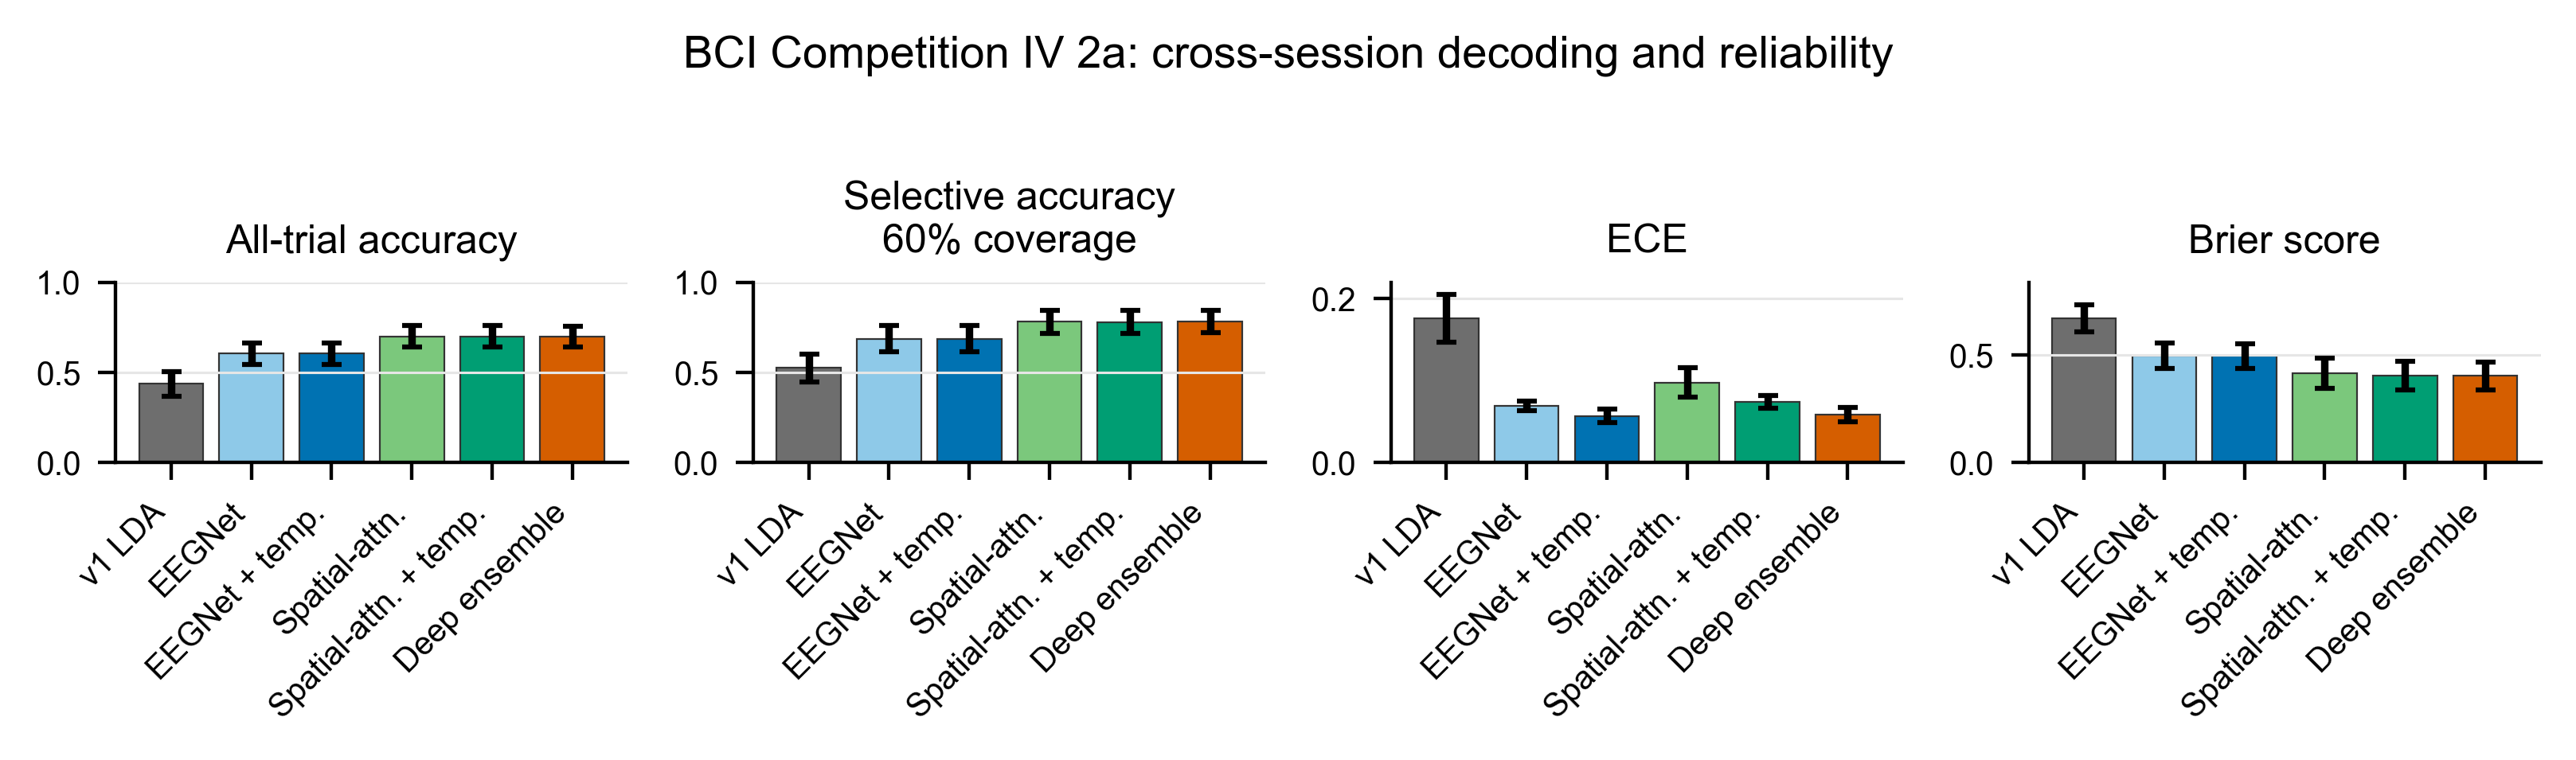
\includegraphics[width=\linewidth]{outputs/v2/paper_artifacts/figures/figure_1_headline_performance_BCI_IV_2a.pdf}
  \caption{\textbf{Headline cross-session performance and reliability.}
  Across nine BCI Competition IV 2a subjects, the v2 deep models improve
  all-trial accuracy and matched 60\%-coverage selective accuracy over the v1
  calibrated LDA baseline. The calibration panels show why accuracy alone is
  insufficient: temperature scaling and ensemble calibration reduce probability
  error as measured by ECE and Brier score. Bars show subject means with
  standard error.}
  \label{fig:headline-performance}
\end{figure}

\begin{figure}[t]
  \centering
  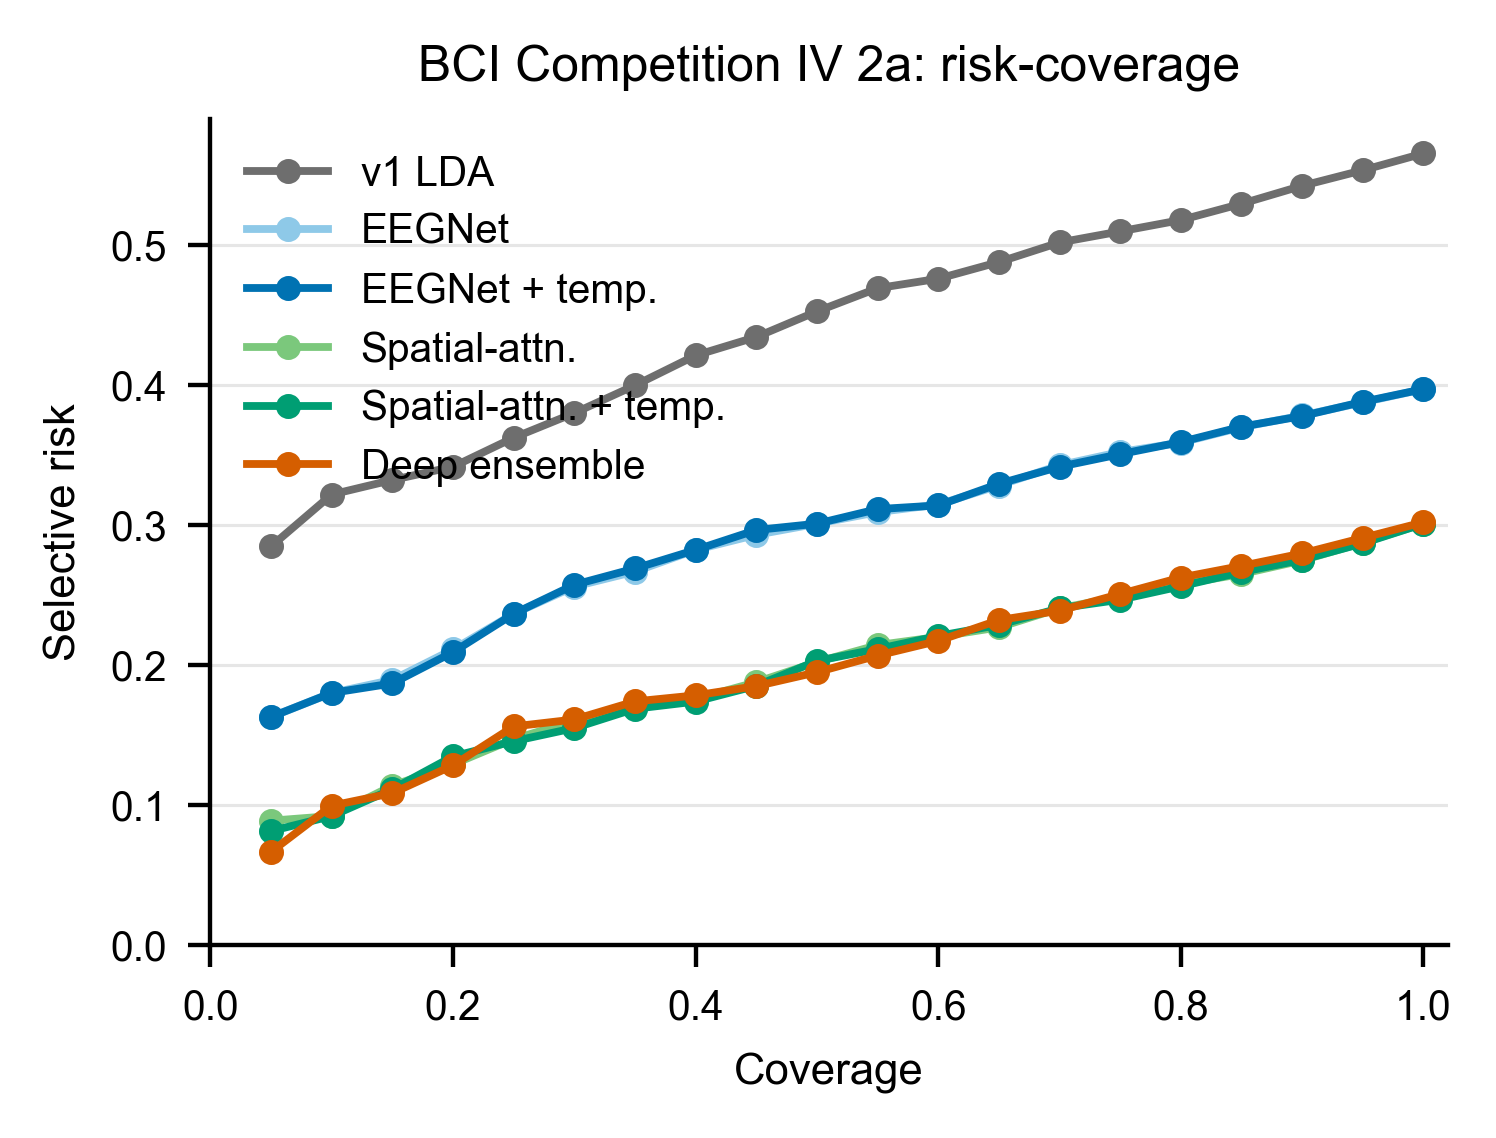
\includegraphics[width=0.72\linewidth]{outputs/v2/paper_artifacts/figures/figure_2_risk_coverage_BCI_IV_2a.pdf}
  \caption{\textbf{Risk-coverage behavior for selective prediction.}
  The curves show the error rate among trials retained at each target coverage.
  A useful assistive-control decoder should move down and to the right: lower
  risk while preserving enough coverage to act. The v2 spatial model and deep
  ensemble maintain lower selective risk than the v1 LDA baseline across the
  operating range.}
  \label{fig:risk-coverage}
\end{figure}

\begin{figure}[t]
  \centering
  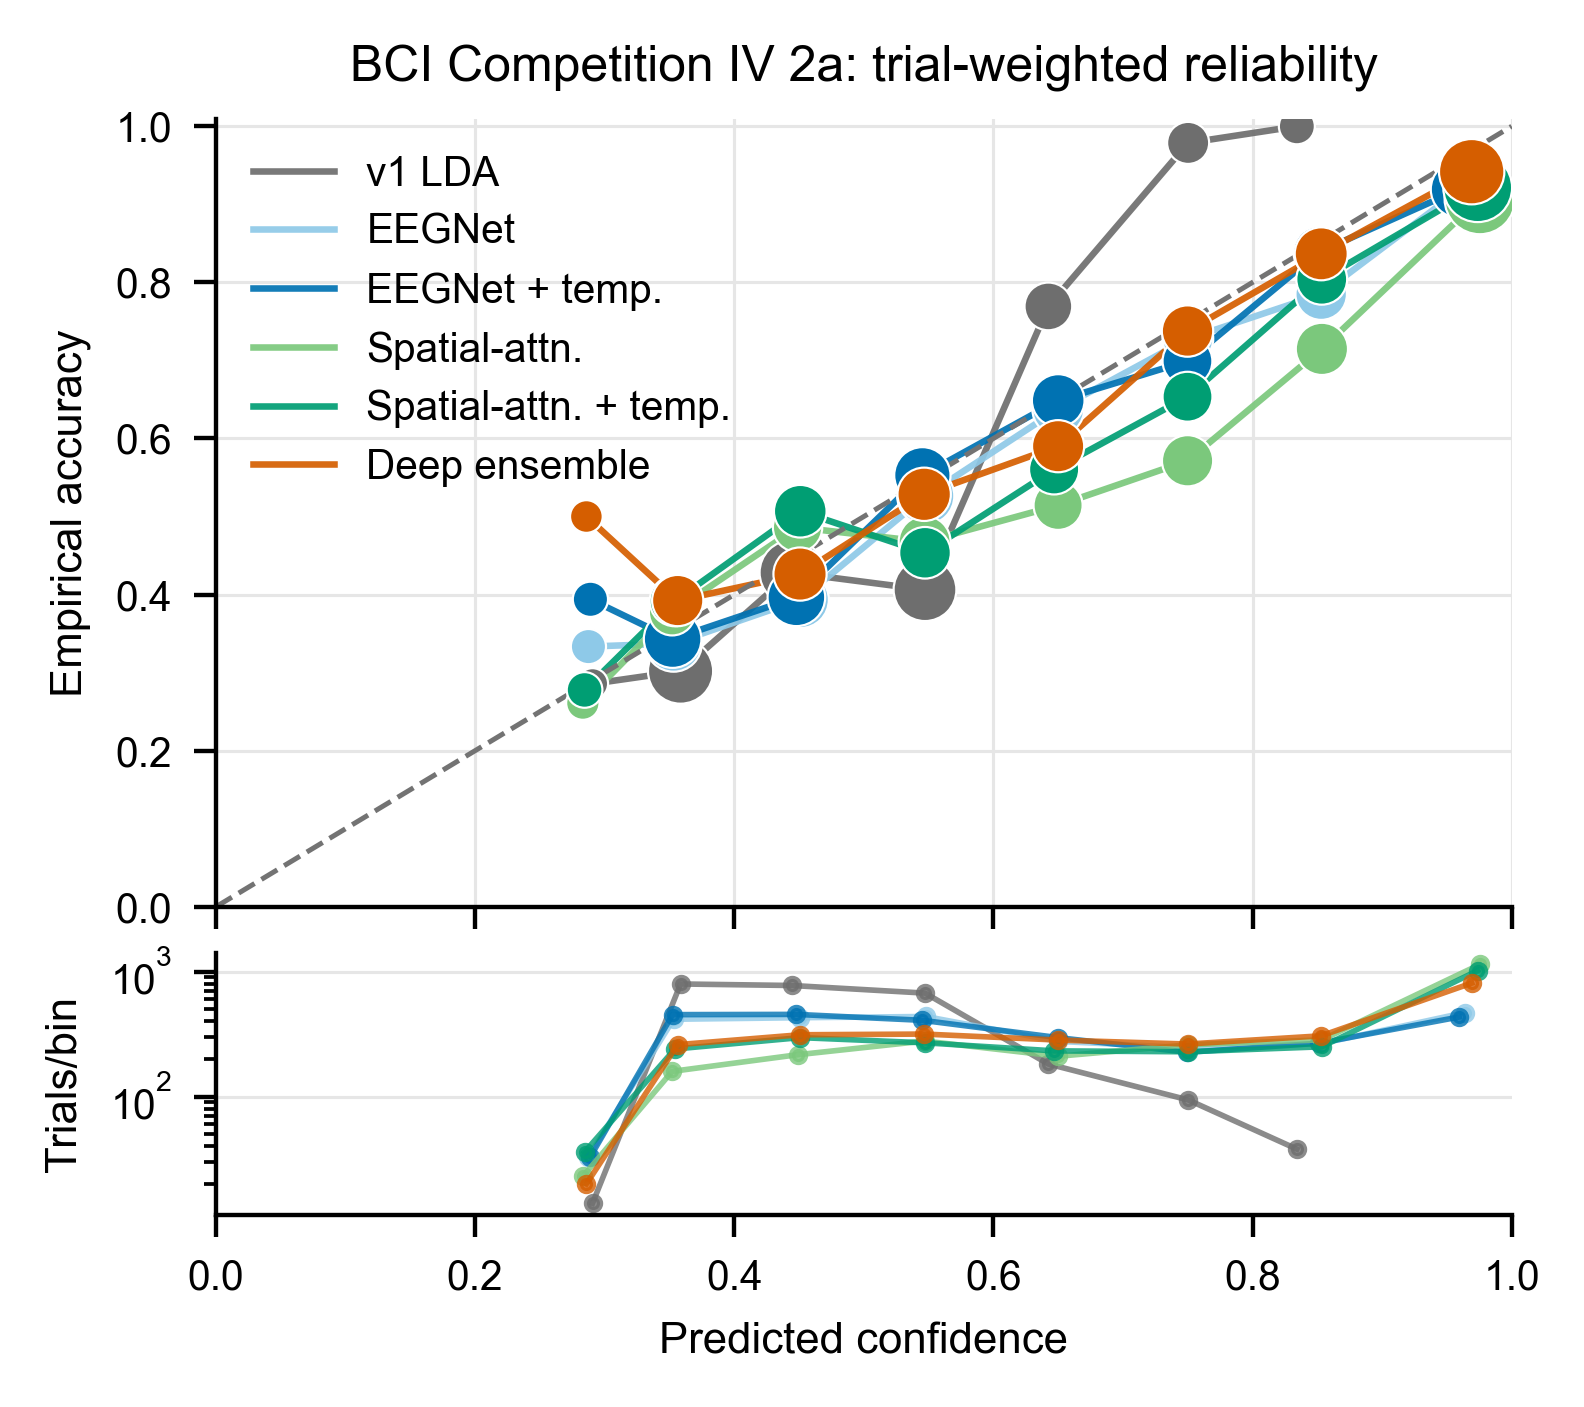
\includegraphics[width=0.72\linewidth]{outputs/v2/paper_artifacts/figures/figure_3_reliability_support_BCI_IV_2a.pdf}
  \caption{\textbf{Trial-weighted reliability with confidence-bin support.}
  Points compare predicted confidence with empirical accuracy, while marker
  size and the lower panel report how many trials fall in each bin. This is the
  critical correction to the naive reliability plot: sparse high-confidence
  bins from v1 LDA should not be interpreted as robust calibration. The v2
  models place many more trials in high-confidence regions while preserving
  substantially better accuracy.}
  \label{fig:reliability-support}
\end{figure}

\begin{figure}[t]
  \centering
  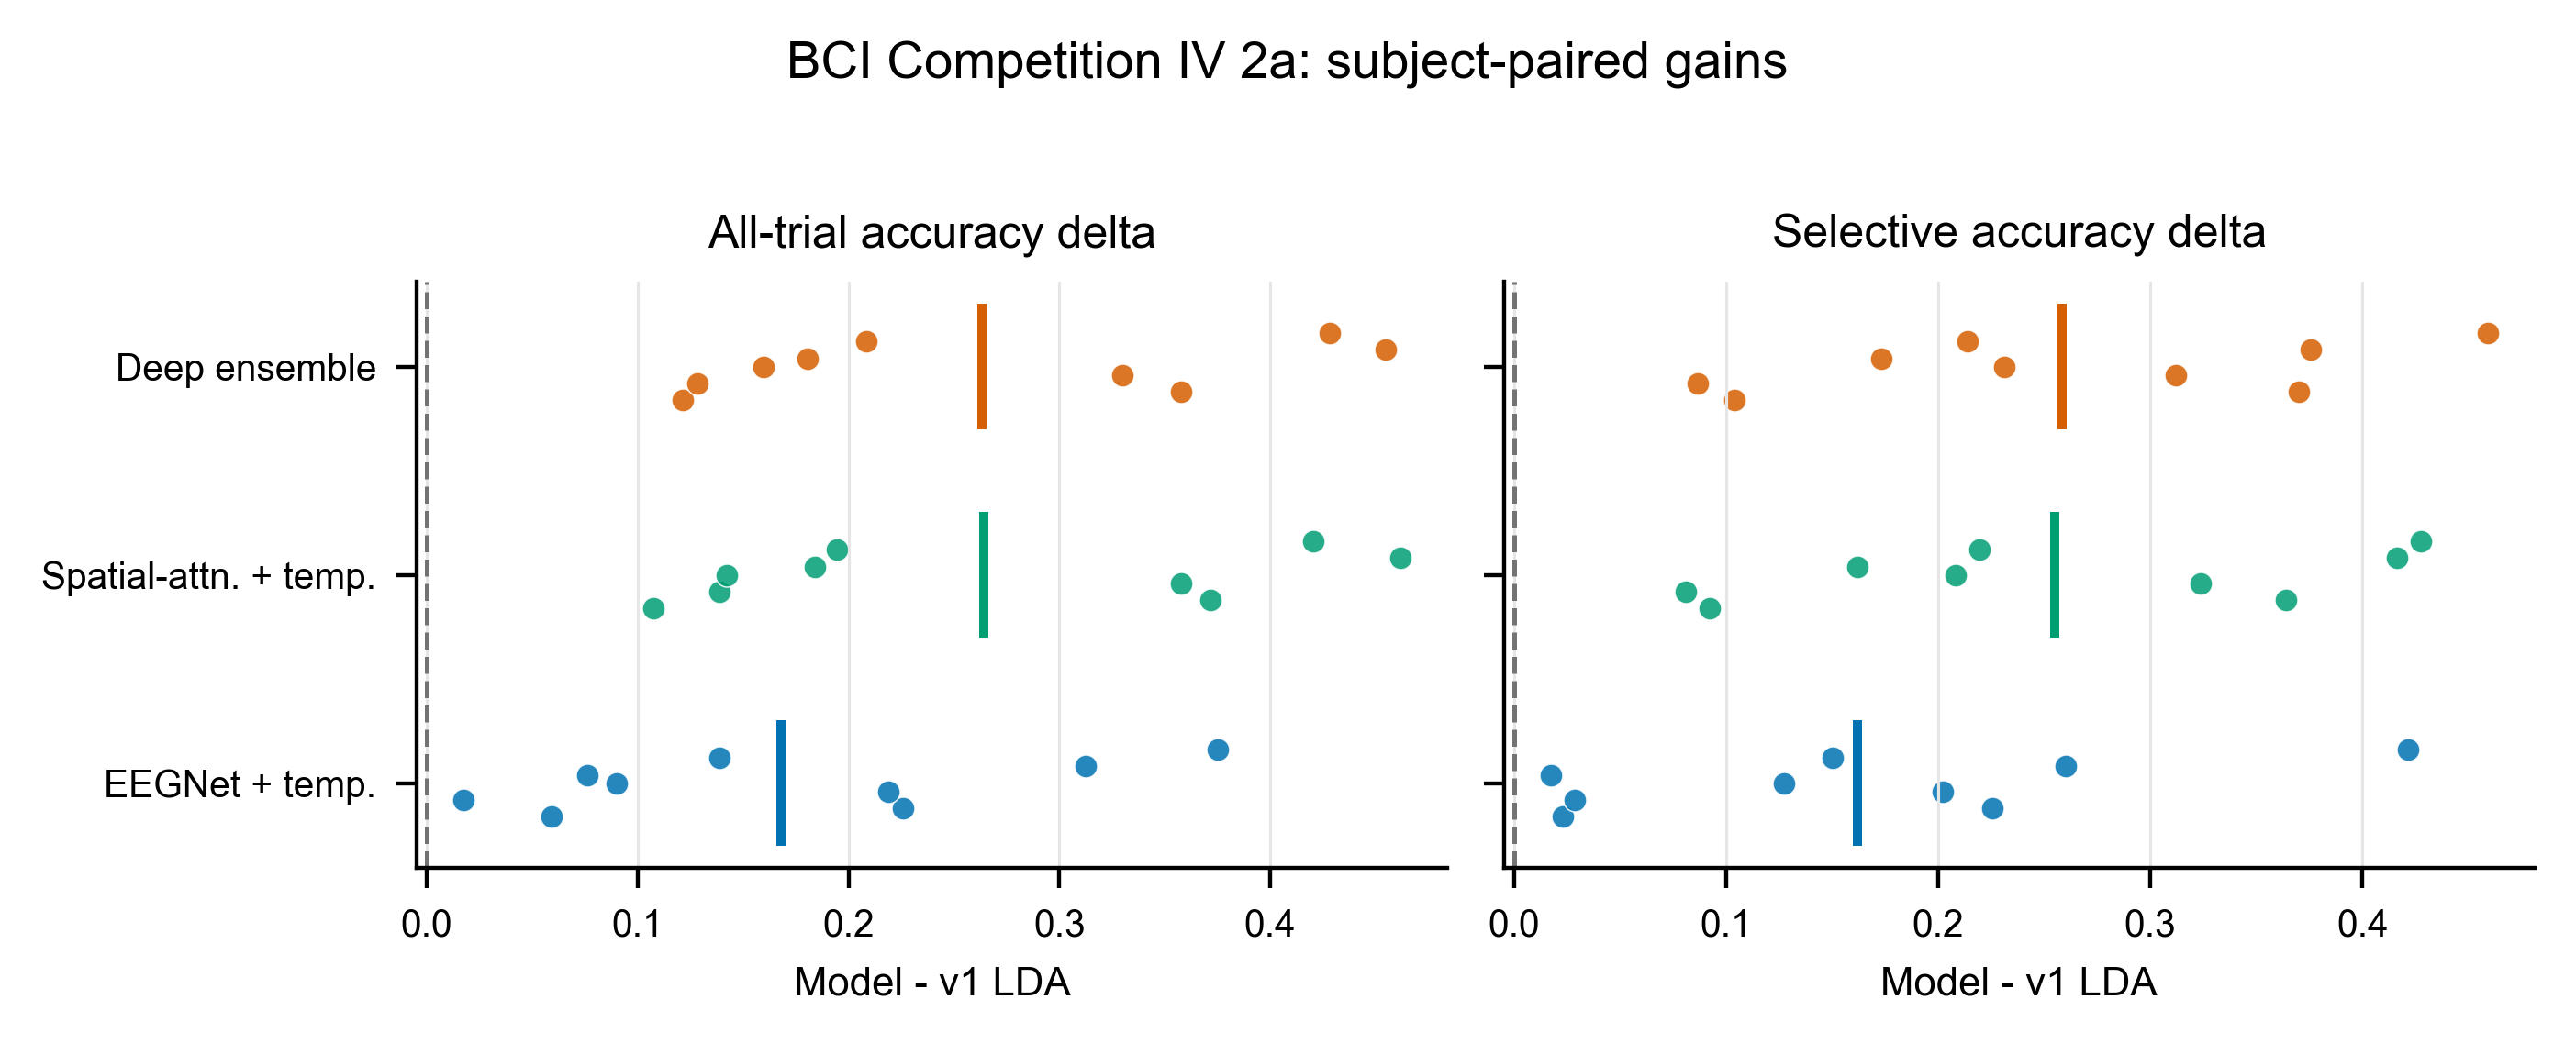
\includegraphics[width=0.86\linewidth]{outputs/v2/paper_artifacts/figures/figure_4_subject_deltas_BCI_IV_2a.pdf}
  \caption{\textbf{Subject-paired gains relative to v1 LDA.}
  Each dot is one subject's improvement over the v1 LDA baseline, and the
  vertical line marks the mean paired delta for each v2 model. This figure
  shows that the headline improvement is not driven by a single subject:
  spatial-attention and deep ensemble models improve both all-trial and
  selective accuracy for most subjects under the same held-out-session
  protocol.}
  \label{fig:subject-deltas}
\end{figure}

\begin{figure}[t]
  \centering
  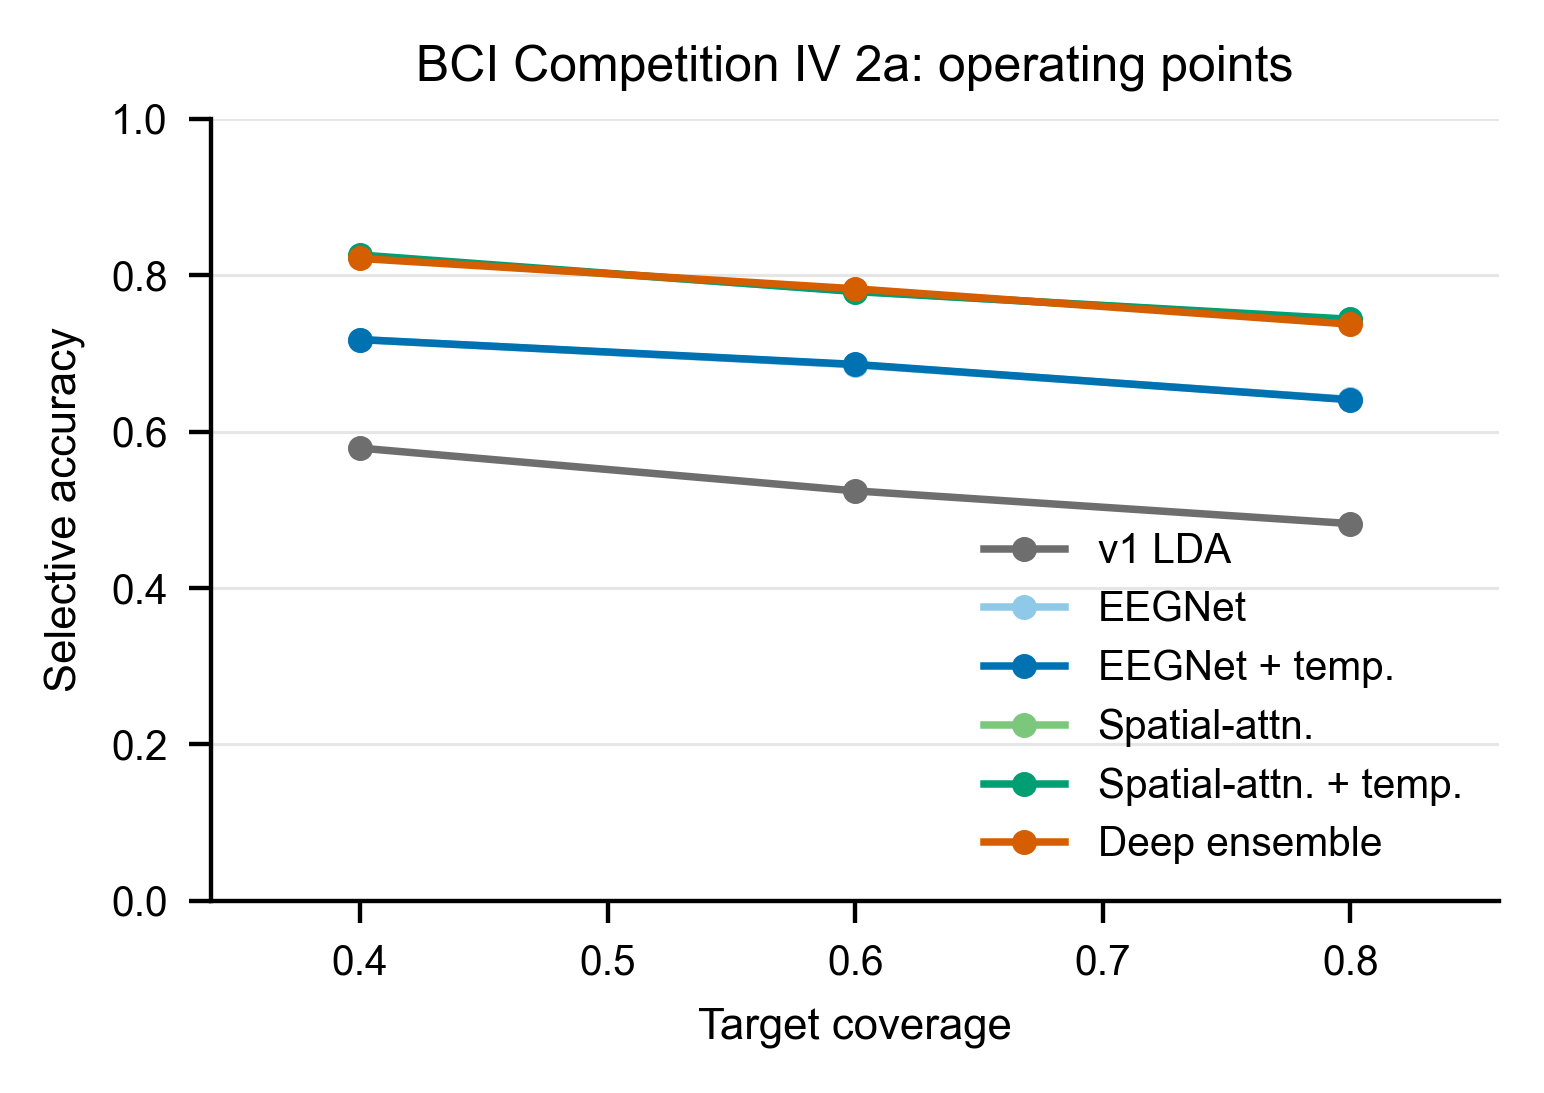
\includegraphics[width=0.72\linewidth]{outputs/v2/paper_artifacts/figures/figure_5_coverage_sweep_BCI_IV_2a.pdf}
  \caption{\textbf{Selective accuracy at practical operating coverages.}
  The 40\%, 60\%, and 80\% operating points summarize how each decoder behaves
  as the system is allowed to abstain more or less often. This supports the
  paper's reliability claim directly: v2 is not only more accurate on all
  trials, but remains stronger when evaluated as a selective controller at
  matched coverage.}
  \label{fig:coverage-sweep}
\end{figure}

\subsection{Why the Corrected Reliability Figure Matters}

An unweighted reliability diagram can make v1 LDA appear unusually strong in
high-confidence bins because some high-confidence bins contain very few trials.
The v2 figure aggregates confidence bins by trial count rather than by subject
row. It also plots the number of trials per bin. This better supports the
paper's claim: v1 LDA can occasionally be accurate when very confident, but
the v2 deep models cover many more trials at high confidence while maintaining
substantially better all-trial and selective performance.

\subsection{Reproducible Artifacts}

The v2 run writes:
\begin{itemize}
  \item \texttt{subject\_metrics.csv},
  \item \texttt{aggregate\_metrics.csv},
  \item \texttt{risk\_coverage.csv},
  \item \texttt{reliability\_diagram\_bins.csv},
  \item \texttt{coverage\_sweep.csv},
  \item \texttt{ablation\_summary.csv}.
\end{itemize}
The paper artifact script additionally writes publication-ready PNG/PDF
figures and two compact table files:
\begin{itemize}
  \item \texttt{headline\_summary\_table.csv},
  \item \texttt{coverage\_sweep\_summary\_table.csv}.
\end{itemize}

\subsection{External Validation and Stress Tests}

The paper-facing validation now includes three stress tests beyond the primary
nine-subject BCI IV 2a run. First, a local BCI Competition IIIa loader
evaluates the same LDA reliability policy on three additional four-class
motor-imagery subjects. On this independent local benchmark, LDA achieves
\(0.659\) all-trial accuracy and \(0.769\) selective accuracy at \(0.614\)
observed coverage.

Second, MOABB validation was expanded from smoke tests to five subjects each
from Cho2017, PhysionetMI, and BNCI2014\_001. Cho2017 reaches \(0.640\)
all-trial accuracy and \(0.724\) selective accuracy with low ECE (\(0.058\)).
BNCI2014\_001 reaches \(0.650\) all-trial accuracy and \(0.692\) selective
accuracy with ECE \(0.102\). PhysionetMI is weaker, with \(0.560\) all-trial
accuracy, \(0.600\) selective accuracy, and ECE \(0.203\). The external
datasets therefore support the reliability framing but not a universal
performance claim.

Third, ablations test whether the reliability result depends on one arbitrary
confidence mechanism. In the local IIIa/IV 2a LDA slice, maximum probability
outperforms margin and entropy at matched 60\% coverage. In a focused
two-subject, 10-epoch deep-ensemble calibration ablation, post-ensemble
temperature scaling gives the strongest probability quality: ECE falls from
\(0.137\) with no temperature scaling to \(0.072\), while matched-coverage
selective accuracy remains approximately stable. This supports calibrating
the ensemble output rather than relying only on per-model calibration.

\subsection{Controller Replay}

Saved probability streams are replayed through a simple FIRE/HOLD controller
with confidence hysteresis and a three-of-five debounce rule. This does not
claim real-time prosthetic control; it translates classifier outputs into
device-facing safety metrics. The balanced controller
\((t_{\mathrm{on}}=0.60, t_{\mathrm{off}}=0.55)\) exposes the tradeoff:
Cho2017 averages \(0.391\) fire coverage, \(0.177\) wrong-fire rate, and
\(0.214\) safe-fire rate, while BNCI2014\_001 averages \(0.136\) fire
coverage, \(0.060\) wrong-fire rate, and \(0.076\) safe-fire rate. A stricter
\((0.80,0.75)\) controller is safer but usually too conservative, often
producing no fires. The conclusion is therefore measured: selective prediction
improves the command stream, but controller thresholds still need user- or
dataset-specific tuning before deployment claims.

\section{Conclusion}

M.I.N.D. v2 strengthens the original reliability-aware BCI framework with
modern deep backbones while preserving the central methodological constraint:
no held-out evaluation labels are used for adaptation, calibration, threshold
selection, or ensemble weighting. The result is a stronger and more credible
paper story. v2 substantially improves accuracy over the classical LDA
baseline, improves selective accuracy at matched coverage, and reports
calibration metrics and risk-coverage curves that directly support the
assistive-control claim.

The most defensible contribution is therefore not simply that a deep model is
more accurate. It is that a modern EEG decoding system can be evaluated as a
selective, probability-aware controller under realistic cross-session shift,
with enough saved artifacts to audit the reliability claim. The external and
controller-replay results strengthen the evaluation story while also exposing
the remaining limitation: reliable abstention is promising, but safe firing
requires tighter threshold calibration and expert review.

\end{document}
